\section{What a recovery curve measures}
\label{sec:blind}

An earlier internal report justified the cell-count rule using a recovery
curve: generate samples at a requested composition and expression shift, then
compare the estimated and requested intrinsic terms. Recovery ratios were
1.00--1.07 where the rule returned an estimate on the reference draw and
0.86--1.18 on the pooled draw, with dispersion decreasing as cell count grew
(Figure~\ref{fig:generator}).

The estimator in this oracle arm applies Equation~\ref{eq:kitagawa} to the
draw's own realised summaries. Across 1{,}711{,}200 replicates of four sweeps on
two cohorts, $\max|\hat\imath-i_{\mathrm{realised}}|=0$. Thus its recovery ratio
is exactly $i_{\mathrm{realised}}/i_{\mathrm{parametric}}$: the realised
reference divided by the requested intrinsic term. The curve describes the
sampling performance of that reference but does not directly test the
abstention rule.

\begin{figure}[htbp]
\centering
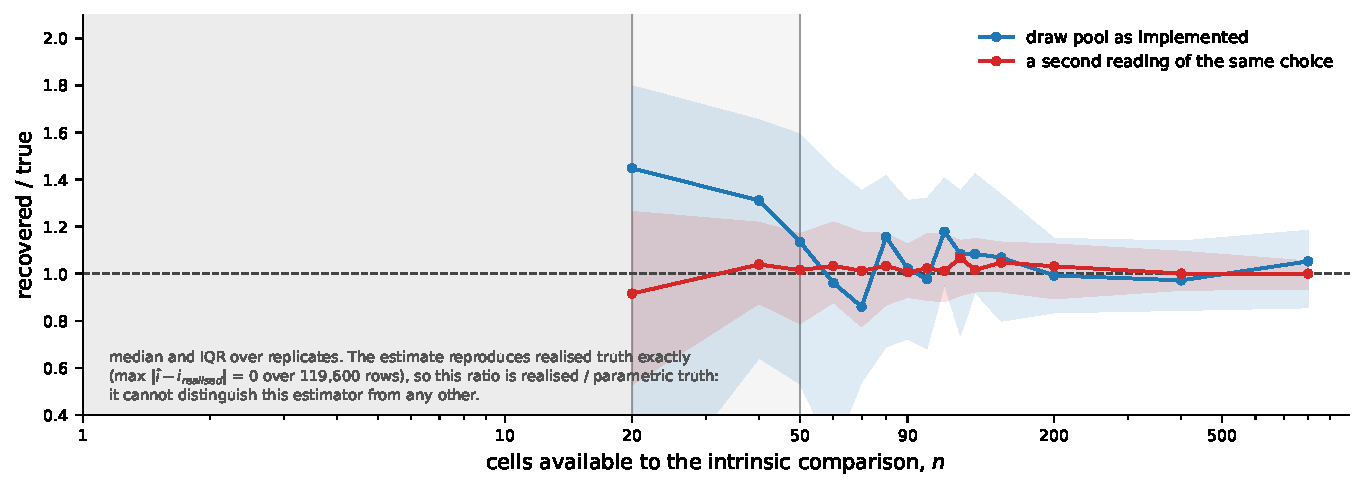
\includegraphics[width=\linewidth]{figures/fig3_generator_statistic.pdf}
\caption{Single-cell recovery ratios at the detectable effect, shown as median
and IQR over 50 replicates for two draw pools. The oracle estimate reproduces
the realised intrinsic reference exactly across all 89{,}700 non-null
replicates in this sweep and 1{,}283{,}400 across four sweeps. The curves therefore
also describe realised over requested truth. The remaining 29{,}900 replicates of this
sweep's 119{,}600 (427{,}800 of 1{,}711{,}200 across four sweeps) have a zero
requested intrinsic term,
so their recovery ratio is undefined. Appendix~\ref{app:generator} compares
the draw pools and explains the constant ratio at the zero-cell grid point.}
\label{fig:generator}
\end{figure}

\paragraph{The general form.}
Let $D$ be a simulated draw requested at parameter $\theta$. Pre-specify an
observed-data reference $T(D)=h(S(D))$, where $S$ denotes summaries of the draw.
We call $T(D)$ the \emph{realised reference}; it need not be a realised causal
effect. If the estimate uses the same functional,
$\hat\theta(D)=h(S(D))$, then, for $\theta\ne0$,
\begin{mdframed}[linewidth=0.5pt,innertopmargin=4pt,innerbottommargin=4pt,nobreak=true]
\[
\frac{\hat\theta(D)}{\theta}=\frac{T(D)}{\theta},
\qquad r(D)=\hat\theta(D)-T(D)\equiv0.
\]
\begin{center}
\texttt{r = estimate[valid] - reference[valid]}\\
\texttt{max\_residual = np.max(np.abs(r))}
\end{center}
\end{mdframed}
Here \texttt{valid} marks paired finite outputs; report excluded draws and do
not compute the maximum if none remain. A maximum below an explicitly chosen
tolerance in outcome units flags numerical equality for investigation.
Only an algebraic argument establishes an identity. Sharing summaries alone
is insufficient: different functions of the same summaries need not agree.

\paragraph{Equality identifies redundancy.}
The recovery curve still measures sampling performance relative to $\theta$.
It cannot distinguish algebraically equivalent implementations or, by itself,
validate interval coverage or an abstention threshold. Even a correctly
implemented sample mean equals its empirical-mean reference. We use ``blind''
only for redundancy relative to a specified reference, not as a verdict on
statistical validity. Our oracle wiring is an observed feature of this
pipeline, not evidence about its prevalence in virtual-control-arm practice.

\paragraph{A control separating equality from performance.}
To test this distinction directly, a separate simulation fixes the reference
before evaluating any estimator: for 200 independent observations
$Y_i\sim\mathcal N(\theta,1)$, set $T(D)=\bar Y$. We evaluate four procedures
at $\theta=0$ and $0.5$, with 2{,}000 replicates per effect. The baseline
reports the full-sample mean with a normal 95\% interval using the sample
standard deviation. A second procedure keeps that point estimate but quarters
the interval half-width. A third adds a known bias of $0.5$ to the baseline
point and interval. The fourth uses every other observation, selected before
seeing outcomes, with its own mean and standard error. This half-sample
estimate shares observations with the full-sample reference; it is not
independent of $T(D)$.

\begin{table}[htbp]
\centering\small
\caption{Equality and statistical performance in the clean control. All
2{,}000 outputs per row are finite. Residuals compare points with the
pre-specified full-sample mean; bias, RMSE and coverage compare with the
requested $\theta$. The nominal coverage is 95\%.}
\label{tab:cleancontrol}
\begin{tabular}{@{}clrrrr@{}}
\toprule
$\theta$ & procedure & $\max|r|$ & bias & RMSE & coverage \\
\midrule
$0$ & Full-sample mean & $0$ & $-0.0008$ & $0.0710$ & $94.60\%$ \\
 & Same point, narrow interval & $0$ & $-0.0008$ & $0.0710$ & $35.95\%$ \\
 & Mean plus $0.5$ & $0.5000$ & $0.4992$ & $0.5042$ & $0.00\%$ \\
 & Half-sample mean & $0.2883$ & $0.0004$ & $0.0994$ & $95.00\%$ \\
\midrule
$0.5$ & Full-sample mean & $0$ & $0.0001$ & $0.0710$ & $95.40\%$ \\
 & Same point, narrow interval & $0$ & $0.0001$ & $0.0710$ & $36.30\%$ \\
 & Mean plus $0.5$ & $0.5000$ & $0.5001$ & $0.5052$ & $0.00\%$ \\
 & Half-sample mean & $0.2686$ & $-0.0017$ & $0.1015$ & $94.20\%$ \\
\bottomrule
\end{tabular}
\end{table}

Table~\ref{tab:cleancontrol} puts adequate and inadequate intervals in the same
zero-residual class. Conversely, departure contains both the unbiased
half-sample mean and the deliberately biased estimate. Coverage Monte Carlo
standard errors are at most 1.08 percentage points. Neither residual class
certifies performance, even with a reference declared in advance. At the
null, differences remain well-defined although recovery ratios do not.

\paragraph{A stratified patient simulator.}
For stratum counts $n_g$, total sample size $n$, and observed arm means
$\bar Y_{ag}$, define
\[
T(D)=\sum_g\frac{n_g}{n}(\bar Y_{1g}-\bar Y_{0g}).
\]
Saturated G-computation \citep{robins1986} calculates this contrast directly.
IPW with empirical propensities $\hat p_g=n_{1g}/n_g$ also equals it: each
stratum's treated weighted sum divided by $n$ is
$(n_g/n)\bar Y_{1g}$, and likewise for controls. This requires nonempty arms
within each stratum and these specific weights. It is not an equivalence for
arbitrary outcome or propensity models. The reference is an observed contrast,
not the finite-sample mean of paired potential-outcome differences.

Figure~\ref{fig:trial} evaluates five estimators in three covariate strata with
stratum-dependent treatment probabilities, a homogeneous additive effect
$\theta=3$, and cohorts of 100--5{,}000 patients. Four estimators recover the
requested effect and tighten with cohort size. Two reproduce $T(D)$:
G-computation has exactly zero residual and saturated IPW agrees to numerical
precision. Cross-fitting the IPW propensity \citep{chernozhukov2018} breaks the
equality in this design because each patient's weight is fitted on a different
fold. It remains consistent here, but its nonzero residual establishes only
departure from this reference. The unadjusted contrast is confounded, with a
recovery ratio near 2.4; the recovery curve correctly reveals that error.

Ordinary least squares (OLS) with treatment and additive stratum dummies also
departs from $T(D)$, although it uses every record and is correctly specified
for this homogeneous effect. Standardisation weights strata by prevalence;
OLS uses normalised weights proportional to $n_g\hat p_g(1-\hat p_g)$.
Its residual is smaller than cross-fitted IPW's at every tested cohort size.
Thus the audit concerns a shared functional, not simply a shared sample
(Table~\ref{tab:trial}).

\begin{figure}[htbp]
\centering
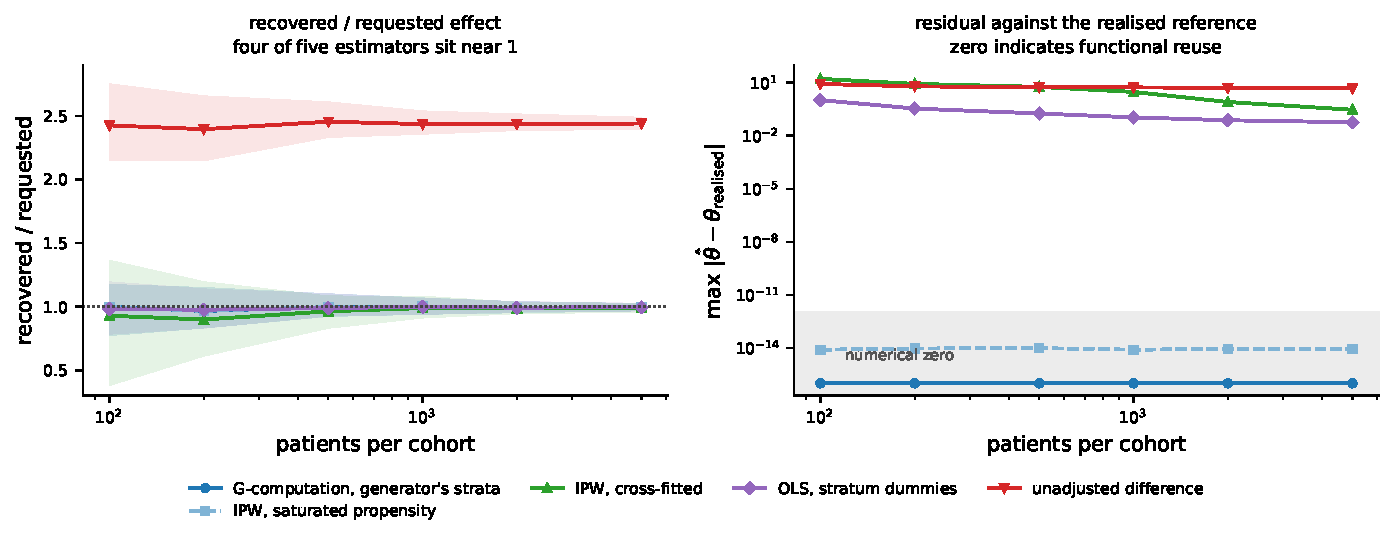
\includegraphics[width=\linewidth]{figures/fig4_trial_recovery.pdf}
\caption{Patient simulation with confounded assignment and requested effect
$\theta=3$. Left: median and IQR of recovery over 200 replicates (197 at the
smallest cohort, after excluding three draws with an empty stratum-arm cell).
Right: residual against the standardised observed-data reference on a log
scale, with a band at machine precision. G-computation and saturated IPW
reproduce the reference. OLS and cross-fitted IPW depart from it while
recovering the requested effect. The unadjusted contrast is confounded.
Departure is not a validity criterion.}
\label{fig:trial}
\end{figure}

\paragraph{Residual scale is descriptive, not an error decomposition.}
Alongside the maximum-residual equality screen, report
\[
\rho=\frac{\mathrm{med}|\hat\theta-T(D)|}
{\mathrm{med}|T(D)-\theta|},
\]
when the denominator is nonzero. OLS has $\rho$ between $0.129$ and $0.137$
across cohorts of 100--5{,}000. Cross-fitted IPW decreases from $1.69$ to
$0.23$; the unadjusted contrast reaches $52.8$ at $n=5{,}000$.
These values compare typical departure with the reference's sampling error.
In $\hat\theta-\theta=(\hat\theta-T)+(T-\theta)$, the terms can covary or
cancel, and medians do not add. Consequently, $\rho$ neither decomposes total
error nor ranks estimator quality. A zero median can conceal nonzero
residuals, which is why the equality screen uses the maximum.

\paragraph{Censoring changes the comparison.}
We repeated the patient experiment with exponential event times, confounded
assignment and administrative censoring: four censoring levels, seven cohort
sizes, and 1{,}200 replicates pooled over 6 seeds per cell. Paired comparisons
exclude non-finite outputs, including event-free cells and Cox fitting failures.
Exclusions occur even at low censoring and remove $463$ of $1{,}200$ draws at
$78\%$ censoring and $n=100$; reported residuals are conditional on valid pairs.

The per-stratum exponential maximum-likelihood estimator uses rates equal to
events divided by exposure, then averages log rate contrasts by stratum
prevalence. Its observed-data reference is that same functional, giving maximum
residual zero in all 28 cells. Against the corresponding latent-time reference,
maximum residuals at $n=3{,}000$ are $0$, $0.061$, $0.144$ and $0.376$ at
$0\%$, $12\%$, $49\%$ and $78\%$ censoring. The worst values across cohort
sizes are $0$, $0.473$, $1.089$ and $1.586$. The estimator is unchanged;
the latent comparison measures a different departure, associated with
information hidden by censoring.

At $49\%$ censoring, the exponential estimator's maximum latent-reference
residual exceeds stratified Cox's in five of seven cohort sizes; at $78\%$, in
six of seven ($0.376$ versus $0.293$ at $n=3{,}000$). Per-replicate inversion
rates are $0.53$--$0.61$. Neither ordering is a quality criterion: a larger
residual cannot be read as a more informative validation. Use an observed-data
reference for the reuse audit, and retain requested parameters and latent
targets for their separate error, coverage and information-loss evaluations.

A restricted-mean survival time (RMST) comparison provides a control.
Its horizon is fixed at $\tau=2$, below every administrative censoring time
in the sweep. Standardised Kaplan--Meier RMST therefore reproduces the empirical
latent truncated-mean contrast to numerical precision across all 28 cells
(maximum residual $2.8\times10^{-15}$ on valid outputs). Censoring has hidden
no information within this horizon. The observation process matters through
its effect on the chosen functional, not simply through the fraction censored.

An independent implementation check compares the repository's stratified
and unadjusted Cox coefficients with \texttt{lifelines.CoxPHFitter} on a
fixed cohort of 1{,}500 patients at the same four censoring horizons. All eight
pairs are finite; the largest absolute difference is $1.4\times10^{-7}$,
below the pre-specified $10^{-5}$ tolerance. This supports agreement of the
implemented fits on this case. It does not validate interval coverage or
characterise convergence across the full simulation grid.

\paragraph{Applying the audit.}
Specify the reference functional, target population and observation process
before examining residuals. Report paired exclusions, the tolerance and maximum
residual separately for each design. Investigate numerical equality
algebraically; do not treat a nonzero residual as evidence of calibration.
At a null requested effect, report differences rather than undefined recovery
ratios. These additions can be made to an existing simulation without changing
the estimator or replacing its performance evaluation.
